\documentclass{article}
\usepackage{amsmath}
\usepackage{tikz}
\usetikzlibrary{angles,quotes}

\begin{document}

The exponent $r \,h(y,\alpha_i)$ in Theorem~\ref{thm:polygon} is the length cut off from the boundary $\partial Q$ by a tangent line to a circle with radius $r$ centered at a vertex that intersects one edge at distance $ry$ from the vertex and the other necessarily at distance $r h(y,\alpha_i)$. For $\alpha_i<\pi/2$ and $y>\cos(\alpha_i)^{-1}$ the picture is different, see Figure~\ref{fig:small-alpha} below.

\begin{figure}[h]
    \centering
    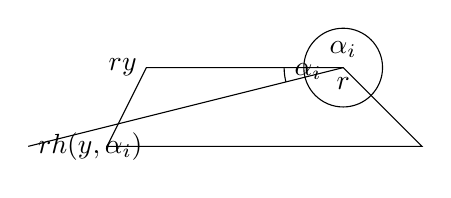
\begin{tikzpicture}
        % Define coordinates
        \coordinate (A) at (0,0);
        \coordinate (B) at (4,0);
        \coordinate (C) at (3,1);
        \coordinate (D) at (2,1);
        \coordinate (E) at (1,1);
        \coordinate (F) at (0.5,1);
        \coordinate (G) at (-1,0);
        
        % Draw the polygon
        \draw (A) -- (B) -- (C) -- (D) -- (E) -- (F) -- cycle;
        
        % Draw the circle
        \draw (C) circle (0.5);
        
        % Draw the tangent lines
        \draw (C) -- (F);
        \draw (C) -- (G);
        
        % Label the points
        \node at (C) [above] {$\alpha_i$};
        \node at (F) [left] {$ry$};
        \node at (G) [right] {$rh(y,\alpha_i)$};
        \node at (C) [below] {$r$};
        
        % Draw the angle
        \pic [draw, angle radius=0.75cm, "$\alpha_i$"] {angle = F--C--G};
    \end{tikzpicture}
    \caption{The exponent $r \,h(y,\alpha_i)$ in Theorem~\ref{thm:polygon} is the length cut off from the boundary $\partial Q$ by a tangent line to a circle with radius $r$ centered at a vertex that intersects one edge at distance $ry$ from the vertex and the other necessarily at distance $r h(y,\alpha_i)$. For $\alpha_i<\pi/2$ and $y>\cos(\alpha_i)^{-1}$ the picture is different.}
    \label{fig:small-alpha}
\end{figure}

\end{document}